%\documentclass[10pt,handout]{beamer}
\documentclass[10pt]{beamer}\usepackage[]{graphicx}\usepackage[]{color}
%% maxwidth is the original width if it is less than linewidth
%% otherwise use linewidth (to make sure the graphics do not exceed the margin)
\makeatletter
\def\maxwidth{ %
  \ifdim\Gin@nat@width>\linewidth
    \linewidth
  \else
    \Gin@nat@width
  \fi
}
\makeatother

\definecolor{fgcolor}{rgb}{0.345, 0.345, 0.345}
\newcommand{\hlnum}[1]{\textcolor[rgb]{0.686,0.059,0.569}{#1}}%
\newcommand{\hlstr}[1]{\textcolor[rgb]{0.192,0.494,0.8}{#1}}%
\newcommand{\hlcom}[1]{\textcolor[rgb]{0.678,0.584,0.686}{\textit{#1}}}%
\newcommand{\hlopt}[1]{\textcolor[rgb]{0,0,0}{#1}}%
\newcommand{\hlstd}[1]{\textcolor[rgb]{0.345,0.345,0.345}{#1}}%
\newcommand{\hlkwa}[1]{\textcolor[rgb]{0.161,0.373,0.58}{\textbf{#1}}}%
\newcommand{\hlkwb}[1]{\textcolor[rgb]{0.69,0.353,0.396}{#1}}%
\newcommand{\hlkwc}[1]{\textcolor[rgb]{0.333,0.667,0.333}{#1}}%
\newcommand{\hlkwd}[1]{\textcolor[rgb]{0.737,0.353,0.396}{\textbf{#1}}}%

\usepackage{framed}
\makeatletter
\newenvironment{kframe}{%
 \def\at@end@of@kframe{}%
 \ifinner\ifhmode%
  \def\at@end@of@kframe{\end{minipage}}%
  \begin{minipage}{\columnwidth}%
 \fi\fi%
 \def\FrameCommand##1{\hskip\@totalleftmargin \hskip-\fboxsep
 \colorbox{shadecolor}{##1}\hskip-\fboxsep
     % There is no \\@totalrightmargin, so:
     \hskip-\linewidth \hskip-\@totalleftmargin \hskip\columnwidth}%
 \MakeFramed {\advance\hsize-\width
   \@totalleftmargin\z@ \linewidth\hsize
   \@setminipage}}%
 {\par\unskip\endMakeFramed%
 \at@end@of@kframe}
\makeatother

\definecolor{shadecolor}{rgb}{.97, .97, .97}
\definecolor{messagecolor}{rgb}{0, 0, 0}
\definecolor{warningcolor}{rgb}{1, 0, 1}
\definecolor{errorcolor}{rgb}{1, 0, 0}
\newenvironment{knitrout}{}{} % an empty environment to be redefined in TeX

\usepackage{alltt}
\usepackage{etex} % helps fix \newdimen error which is cause when ctable is loaded with other packages
\usepackage{comment}
\usepackage{ctable}
\usepackage{amsmath,amsthm,amssymb}
\usepackage{url}
\usepackage{color, colortbl}
\usepackage{tikz}
\usetikzlibrary{shapes.geometric, arrows,shapes.symbols,decorations.pathreplacing}
\tikzstyle{startstop} = [rectangle, rounded corners, minimum width=3cm, minimum height=1cm,text centered, draw=black, fill=red!30,text width=2.0cm]
\tikzstyle{io} = [trapezium, trapezium left angle=70, trapezium right angle=110, minimum width=2cm, minimum height=1cm, text centered, draw=black, fill=blue!30,text width=1.5cm]
\tikzstyle{process} = [rectangle, minimum width=1cm, minimum height=1cm, text centered, draw=black, fill=orange!30,text width=2cm]
\tikzstyle{decision} = [diamond, minimum width=2cm, minimum height=1cm, text centered, draw=black, fill=green!30]
\tikzstyle{arrow} = [thick,->,>=stealth]
\tikzstyle{both} = [thick,<->,>=stealth, red]

\tikzset{myshade/.style={minimum size=.4cm,shading=radial,inner color=white,outer color={#1!90!gray}}}
\newcommand\mycirc[1][]{\tikz\node[circle,myshade=#1]{};}
\newcommand\myrect[1][]{\tikz\node[rectangle,myshade=#1]{};}
\newcommand\mystar[1][]{\tikz\node[star,star points=15,star point height=2pt,myshade=#1]{};}
\newcommand\mydiamond[1][]{\tikz\node[diamond,myshade=#1]{};}
\newcommand\myellipse[1][]{\tikz\node[ellipse,myshade=#1]{};}
\newcommand\mykite[1][]{\tikz\node[kite,myshade=#1]{};}
\newcommand\mydart[1][]{\tikz\node[dart,myshade=#1]{};}
\newcommand\mycloud[1][]{\tikz\node[cloud,myshade=#1]{};}

%\usepackage{subcaption}
\usepackage{subfig}
%\usepackage{caption}

\mode<presentation>
\usetheme{Hannover}
\usecolortheme{rose}
\setbeamertemplate{navigation symbols}{}
\setbeamertemplate{footline}[frame number]
\setbeamertemplate{caption}[numbered]
\setbeamertemplate{frametitle}[default][left]

\usepackage[]{hyperref}
\hypersetup{
    unicode=false,          
    pdftoolbar=true,        
    pdfmenubar=true,        
    pdffitwindow=false,     % window fit to page when opened
    pdfstartview={FitH},    % fits the width of the page to the window
    pdftitle={Reproducible Research},    % title
    pdfauthor={Sahir Rai Bhatnagar},     % author
    pdfsubject={Subject},   % subject of the document
    pdfcreator={Sahir Rai Bhatnagar},   % creator of the document
    pdfproducer={Sahir Rai Bhatnagar}, % producer of the document
    pdfkeywords={}, % list of keywords
    pdfnewwindow=true,      % links in new window
    colorlinks=true,       % false: boxed links; true: colored links
    linkcolor=red,          % color of internal links (change box color with linkbordercolor)
    citecolor=blue,        % color of links to bibliography
    filecolor=black,      % color of file links
    urlcolor=cyan           % color of external links
}
\IfFileExists{upquote.sty}{\usepackage{upquote}}{}
\begin{document}










\title[RR: Intro to \texttt{knitr}]{Reproducible Research}
\subtitle{An Introduction to \texttt{knitr}}

\author[]{Sahir Bhatnagar%
\thanks{sahir.bhatnagar@mail.mcgill.ca%
}}

\date{May 28, 2014}

%\makebeamertitle

\maketitle

\begin{frame}{Acknowledgements}
% \hspace*{-1.9cm}\parbox[t]{\textwidth}
%\frametitle{Acknowledgements}
\begin{columns}[c] % The "c" option specifies centered vertical alignment while the "t" option is used for top vertical alignment

\column{.45\textwidth} % Left column and width

\begin{itemize}
%\scriptsize
\item Dr. Erica Moodie
\item Maxime Turgeon, Kevin McGregor, Greg Voisin
\item You
\end{itemize}

\column{.45\textwidth} % Right column and width
\begin{figure}

\includegraphics[width=0.6\columnwidth]{eboh50.pdf}\\[5mm]

\includegraphics[width=1.0\columnwidth]{crm.png}
%\includegraphics[width=0.7\columnwidth]{Logo-LUDMER.jpg}
\end{figure}

\end{columns}
\end{frame}



\begin{frame}{Disclaimer}
\begin{figure}

\includegraphics[width=1.0\columnwidth]{rstudio.png}\\[5mm]

\includegraphics[width=0.2\columnwidth]{rlogo.png}\\[5mm]

\includegraphics[width=0.2\columnwidth]{LaTeX_logo.png}
\end{figure}

\textit{I don't work for, nor am I an author of any of these packages. I'm just a messenger.}

\end{frame}

\begin{frame}{Disclaimer}

\begin{itemize}
\item Material for this tutorial comes from many sources. For a complete list see:  \href{https://github.com/sahirbhatnagar/knitr-tutorial}{https://github.com/sahirbhatnagar/knitr-tutorial}
\item Alot of the content in these slides are based on these two books
\end{itemize}

\begin{columns}[c] % The "c" option specifies centered vertical alignment while the "t" option is used for top vertical alignment
\column{.45\textwidth} % Left column and width
\begin{figure}
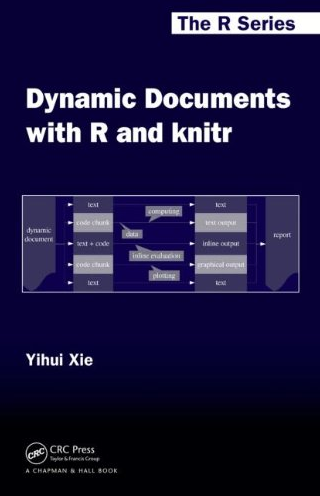
\includegraphics[width=0.6\columnwidth]{yihui.png}
\end{figure}

\column{.45\textwidth} % Right column and width
\begin{figure}
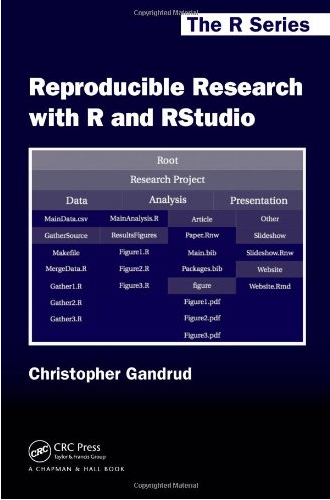
\includegraphics[width=0.6\columnwidth]{chris.png}
\end{figure}
\end{columns}

\end{frame}


\begin{frame}{Eat Your Own Dog Food}

\begin{itemize}
\item These slides are reproducible
\item Source code: \href{https://github.com/sahirbhatnagar/knitr-tutorial}{https://github.com/sahirbhatnagar/knitr-tutorial}
\end{itemize}

\end{frame}


\section{Reproducible Research}

\subsection{What?}

\begin{frame}

\frametitle{What is Science Anyway?}

\pause
\begin{block}{According to the American Physical Society:}
\emph{Science is the systematic enterprise of gathering knowledge about the universe and organizing and condensing that knowledge into \textbf{testable} laws and theories. The \textbf{success and credibility of science} are anchored in the \textbf{willingness} of scientists to \textbf{expose their ideas} and results to \textbf{independent testing} and \textbf{replication} by other scientists}
\end{block}

\end{frame}

%%%%%%%%%%%%%%%%%%%%%%%%%%%%%%%%%%%%%%%%%%%%%%%%%%%%%%%%%%%%%%%%%%%%%%%%%%%%%%%%%%%%%%%%%%%%%
\begin{frame}

\frametitle{RR: A Minimum Standard to Verify Scientific Findings}

\pause
\begin{block}{Reproducible Research (RR) in Computational Sciences}
\emph{The data and the code used to make a finding are available and they are sufficient for an independent researcher to recreate the finding}
\end{block}

\end{frame}

%%%%%%%%%%%%%%%%%%%%%%%%%%%%%%%%%%%%%%%%%%%%%%%%%%%%%%%%%%%%%%%%%%%%%%%%%%%%%%%%%%%%%%%%%%%%%
%%%%%%%%%%%%%%%%%%%%%%%%%%%%%%%%%%%%%%%%%%%%%%%%%%%%%%%%%%%%%%%%%%%%%%%%%%%%%%%%%%%%%%%%%%%%%

\subsection{Why?}

\begin{frame}
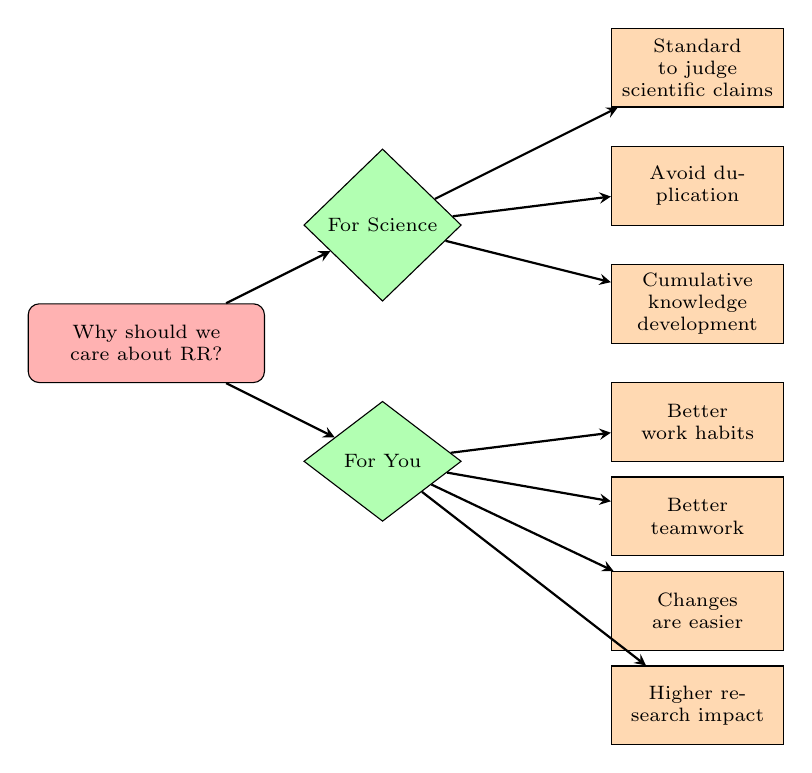
\begin{tikzpicture}
\scriptsize
\node (expr) [startstop] {Why should we care about RR?};
\node (science) [decision, right of=expr, xshift=2cm, yshift=1.5cm] {For Science};
\draw [arrow] (expr) -- (science);
\node (stan) [process, right of=science, xshift=3cm, yshift=2cm] {Standard to judge scientific claims};
\node (dupli) [process, right of=science, xshift=3cm, yshift=0.5cm] {Avoid duplication};
\node (know) [process, right of=science, xshift=3cm, yshift=-1cm] {Cumulative knowledge development};
\draw [arrow] (science) -- (stan);
\draw [arrow] (science) -- (dupli);
\draw [arrow] (science) -- (know);
\pause \node (you) [decision, right of=expr, xshift=2cm, yshift=-1.5cm] {For You};
\draw [arrow] (expr) -- (you);
\node (work) [process, right of=you, xshift=3cm, yshift=0.5cm] {Better work habits};
\node (team) [process, right of=you, xshift=3cm, yshift=-0.7cm] {Better teamwork};
\node (change) [process, right of=you, xshift=3cm, yshift=-1.9cm] {Changes are easier};
\node (soft) [process, right of=you, xshift=3cm, yshift=-3.1cm] {Higher research impact};
\draw [arrow] (you) -- (work);
\draw [arrow] (you) -- (team);
\draw [arrow] (you) -- (change);
\draw [arrow] (you) -- (soft);
\end{tikzpicture}
\end{frame}


\subsection{001-motivating-example}

\begin{frame}{A Motivating Example}
\textit{Demonstrate:} \href{https://github.com/sahirbhatnagar/knitr-tutorial/tree/master/001-motivating-example}{001-motivating-example}
\end{frame}



\section{Getting Started}

\begin{frame}{Tools for Reproducible Research\footnote{\href{http://onepager.togaware.com/}{http://onepager.togaware.com/}}}


\begin{block}{Free and Open Source Software}
\begin{itemize}
\item \texttt{RStudio}: Creating, managing, compiling documents
\item \LaTeX: Markup language for typesetting a document
\item \texttt{R}: Statistical analysis language
\item \texttt{knitr}: Integrate \LaTeX and \texttt{R} code. Based on Prof. Friedrich Leisch's \href{https://www.statistik.lmu.de/~leisch/Sweave/}{\texttt{Sweave}}
\end{itemize}
\end{block}
\end{frame}


\subsection{\LaTeX}

\begin{frame}\frametitle{Comparison}
\begin{columns}[c] % The "c" option specifies centered vertical alignment while the "t" option is used for top vertical alignment

\column{.45\textwidth} % Left column and width
\begin{figure}[h!]
\centering
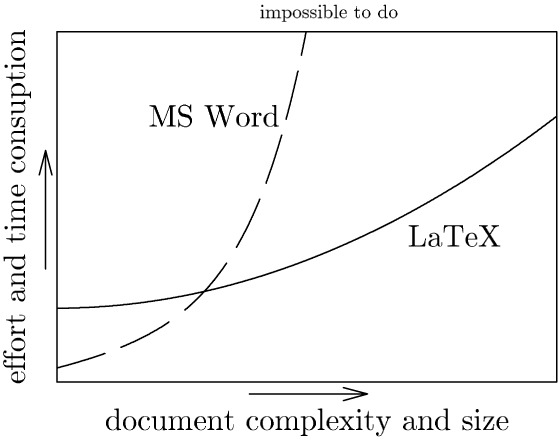
\includegraphics[scale=1, keepaspectratio]{./miktex}
\caption{Comparison}
\label{fig:word}
\end{figure}

\column{.5\textwidth} % Right column and width
\begin{itemize}
\item \LaTeX \, has a greater learning curve
\item Many tasks are very tedious or impossible (most cases) to do in MS Word or Libre Office
\end{itemize}
\end{columns}

\end{frame}

%%%%%%%%%%%%%%%%%%%%%%%%%%%%%%%%%%%%%%%%%%%%%%%%%%%%%%%%%%%%%%%%%%%%%%%%%%%%%%%%%%%%%%%%%%%%%

\begin{frame}\frametitle{The Philosophy behind \LaTeX}
\begin{columns}[c] % The "c" option specifies centered vertical alignment while the "t" option is used for top vertical alignment

\column{.45\textwidth} % Left column and width
\begin{figure}[h!]
\centering
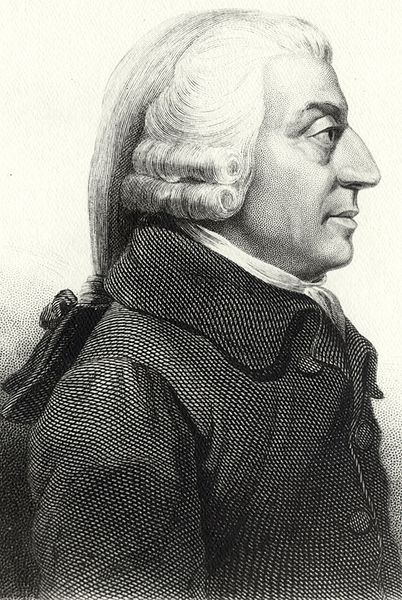
\includegraphics[scale=0.6, keepaspectratio]{./smith}
\small
\caption{Adam Smith, author of \textit{The Wealth of Nations} (1776), in which he conceptualizes the notion of the division of labour}
\label{fig:smith}
\end{figure}

\column{.5\textwidth} % Right column and width
\small
\begin{block}{Division of Labour}
Composition and logical structuring of text is the author's specific contribution to the production of a printed text. Matters such as the choice of the font family, should section headings be in bold face or small capitals? Should they be flush left or centered? Should the text be justified or not? Should the notes appear at the foot of the page or at the end? Should the text be set in one column or two? and so on, is the typesetter's business
\end{block}
\end{columns}

\end{frame}

%%%%%%%%%%%%%%%%%%%%%%%%%%%%%%%%%%%%%%%%%%%%%%%%%%%%%%%%%%%%%%%%%%%%%%%%%%%%%%%%%%%%%%%%%%%%%

\begin{frame}\frametitle{The Genius Behind \LaTeX}

\begin{figure}[h!]
\centering
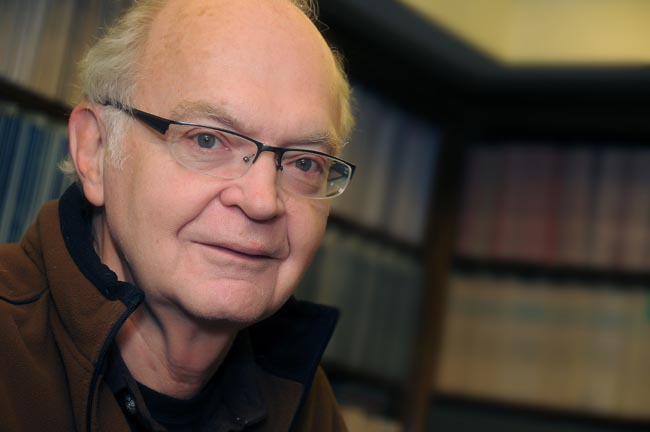
\includegraphics[scale=0.4, keepaspectratio]{./don}
\small
\caption{The \TeX~project was started in 1978 by Donald Knuth (Stanford). He planned for 6 months, but it took him nearly 10 years to complete. Coined the term ``Literate programming'': mixture of code and text segments that are ``human'' readable. Recipient of the Turing Award (1974) and the Kyoto Prize (1996).}
\label{fig:don}
\end{figure}

\end{frame}



\subsection{RStudio}

\begin{frame}\frametitle{Integrated Development Environment (IDE)}
\pause
\begin{figure}[h!]
\centering
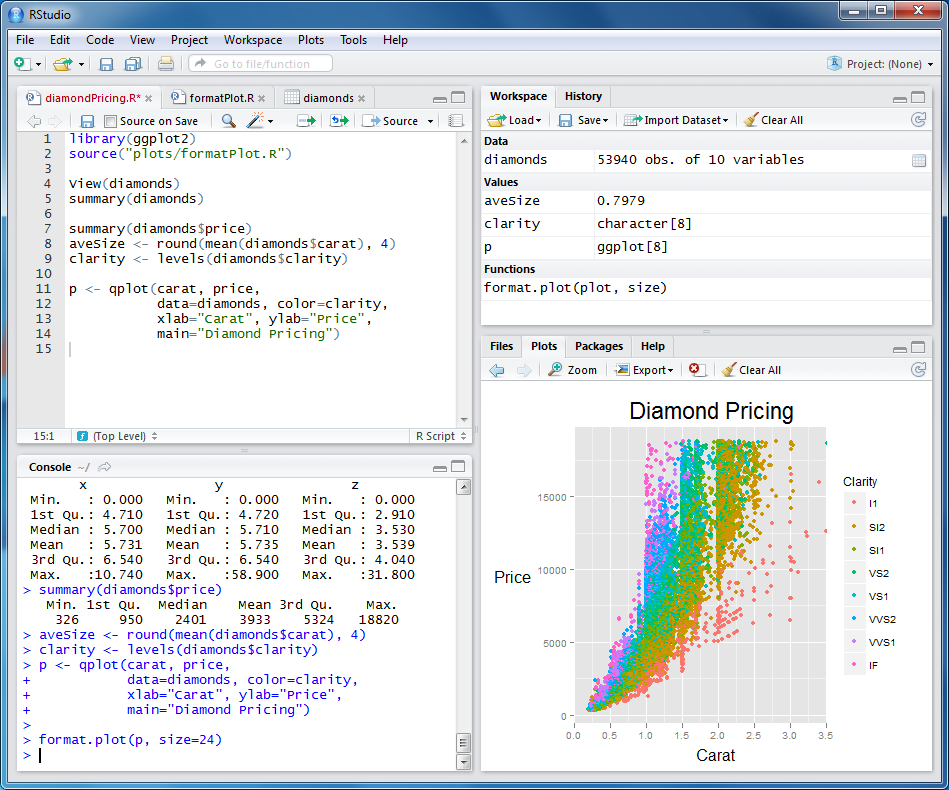
\includegraphics[scale=0.25, keepaspectratio]{./RStudio-Screenshot}
\end{figure}
\textit{Demonstrate:} Explore \texttt{RStudio}, projects and \texttt{.Rprofile}
\end{frame}


\subsection{\texttt{knitr}}

\begin{frame}{What \texttt{knitr} does}
\textbf{\LaTeX} example:

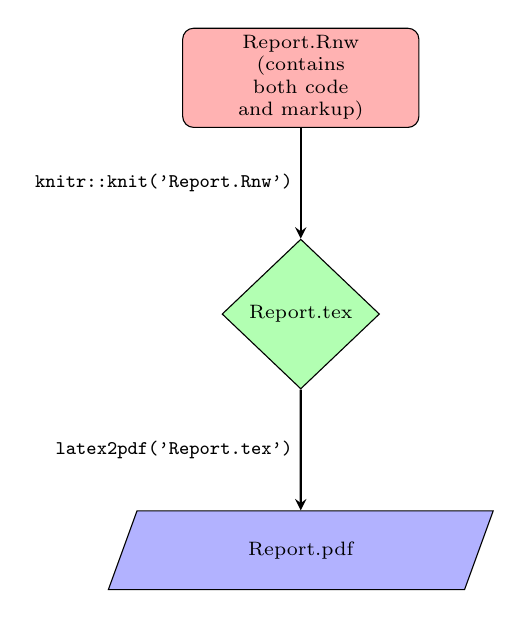
\begin{tikzpicture}
\scriptsize
\node (expr) [startstop] {Report.Rnw (contains both code and markup)};
\node (science) [decision, below of=expr, xshift=0cm, yshift=-2cm] {Report.tex};
\draw [arrow] (expr) -- node[anchor=east]{\texttt{knitr::knit('Report.Rnw')}} (science);
\pause \node (pdf) [io, below of=science, xshift=0cm, yshift=-2cm] {Report.pdf};
\draw [arrow] (science) -- node[anchor=east]{\texttt{latex2pdf('Report.tex')}} (pdf);
\end{tikzpicture}
\end{frame}


\begin{frame}\frametitle{Compiling a \texttt{.Rnw} document}

\begin{block}{The two steps on previous slide can be executed in one command:}
\[ \textrm{\texttt{knitr::knit2pdf()}} \]
\end{block}

or in \texttt{RStudio}:
\begin{figure}[h!]
\centering
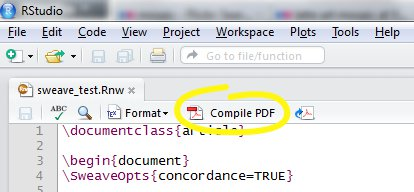
\includegraphics[scale=0.5, keepaspectratio]{./Compile-pdf.jpg}
\end{figure}
%\textit{Demonstrate:} Explore \texttt{RStudio}, projects and \texttt{.Rprofile}
\end{frame}

\begin{frame}\frametitle{Incorporating \texttt{R} code}

\begin{itemize}
\item Insert \texttt{R} code in a \textbf{Code Chunk} starting with $$ << \quad >>= $$
and ending with \begin{center}
{@}
\end{center}
\end{itemize}

In \texttt{RStudio}:
\begin{figure}[h!]
\centering
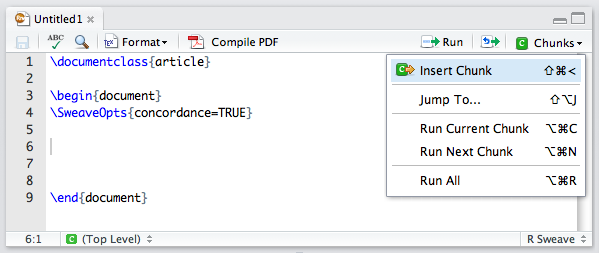
\includegraphics[scale=0.35, keepaspectratio]{./sweave_chunk}
\end{figure}
%\textit{Demonstrate:} Explore \texttt{RStudio}, projects and \texttt{.Rprofile}
\end{frame}

\begin{frame}[fragile]{Example 1}
\begin{knitrout}
\definecolor{shadecolor}{rgb}{0.969, 0.969, 0.969}\color{fgcolor}\begin{kframe}
\begin{verbatim}
<<example-code-chunk-name, echo=TRUE>>=
library(magrittr)
rnorm(50) %>% mean
@
\end{verbatim}
\end{kframe}
\end{knitrout}
produces
\begin{knitrout}
\definecolor{shadecolor}{rgb}{0.969, 0.969, 0.969}\color{fgcolor}\begin{kframe}
\begin{alltt}
\hlkwd{library}\hlstd{(magrittr)}
\hlkwd{rnorm}\hlstd{(}\hlnum{50}\hlstd{)} \hlopt \hlstd{mean}
\end{alltt}
\begin{verbatim}
## [1] 0.031
\end{verbatim}
\end{kframe}
\end{knitrout}
\end{frame}


\begin{frame}[fragile]{Example 2}
\begin{knitrout}
\definecolor{shadecolor}{rgb}{0.969, 0.969, 0.969}\color{fgcolor}\begin{kframe}
\begin{verbatim}
<<example-code-chunk-name2, echo=TRUE, tidy=TRUE>>=
for(i in 1:5){ (i+3) %>% print}
@
\end{verbatim}
\end{kframe}
\end{knitrout}
produces
\begin{knitrout}
\definecolor{shadecolor}{rgb}{0.969, 0.969, 0.969}\color{fgcolor}\begin{kframe}
\begin{alltt}
\hlkwa{for} \hlstd{(i} \hlkwa{in} \hlnum{1}\hlopt{:}\hlnum{5}\hlstd{) \{}
    \hlstd{(i} \hlopt{+} \hlnum{3}\hlstd{)} \hlopt \hlstd{print}
\hlstd{\}}
\end{alltt}
\begin{verbatim}
## [1] 4
## [1] 5
## [1] 6
## [1] 7
## [1] 8
\end{verbatim}
\end{kframe}
\end{knitrout}

\end{frame}


\begin{frame}[fragile]{Example 2.2}
\begin{knitrout}
\definecolor{shadecolor}{rgb}{0.969, 0.969, 0.969}\color{fgcolor}\begin{kframe}
\begin{verbatim}
<<example-code-chunk-name3, echo=FALSE>>=
for(i in 1:5){ (i+3) %>% print}
@
\end{verbatim}
\end{kframe}
\end{knitrout}
produces
\begin{knitrout}
\definecolor{shadecolor}{rgb}{0.969, 0.969, 0.969}\color{fgcolor}\begin{kframe}
\begin{verbatim}
## [1] 4
## [1] 5
## [1] 6
## [1] 7
## [1] 8
\end{verbatim}
\end{kframe}
\end{knitrout}

\end{frame}


\begin{frame}[fragile]{Example 2.3}
\begin{knitrout}
\definecolor{shadecolor}{rgb}{0.969, 0.969, 0.969}\color{fgcolor}\begin{kframe}
\begin{verbatim}
<<example-code-chunk-name4, echo=FALSE, eval=FALSE>>=
for(i in 1:5){ (i+3) %>% print}
@
\end{verbatim}
\end{kframe}
\end{knitrout}
produces


\end{frame}



\begin{frame}[fragile]{\texttt{R} output within the text}
\begin{itemize}
\item Include \texttt{R} output within the text
\item We can do that with ``S-expressions'' using the command \textbackslash \texttt{Sexpr}\{$\ldots$\}
\end{itemize}
\vspace{1cm}

\textbf{Example:} \vspace{0.3cm}

The iris dataset has \textbackslash \texttt{Sexpr}\{\texttt{nrow(iris)}\} rows and \textbackslash \texttt{Sexpr}\{\texttt{ncol(iris)}\} columns
\vspace{0.5cm}

produces \vspace{0.5cm}

The iris dataset has 150 rows and 5 columns


\end{frame}


\begin{frame}[fragile]
\frametitle{Include a Figure}
\scriptsize
\begin{knitrout}
\definecolor{shadecolor}{rgb}{0.969, 0.969, 0.969}\color{fgcolor}\begin{kframe}
\begin{verbatim}
<<fig.ex, fig.cap='Linear Regression',fig.height=3,fig.width=3>>=
plot(mtcars[ , c('disp','mpg')])
lm(mpg ~ disp , data = mtcars) %>%
abline(lwd=2)
@
\end{verbatim}
\end{kframe}
\end{knitrout}
\begin{knitrout}
\definecolor{shadecolor}{rgb}{0.969, 0.969, 0.969}\color{fgcolor}\begin{figure}

{\centering 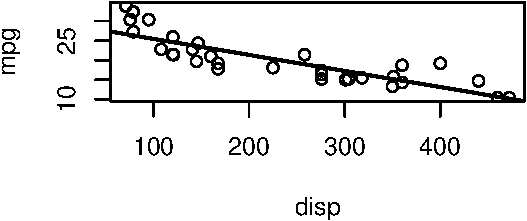
\includegraphics[width=\maxwidth]{figure/slr7-1} 

}

\caption[Linear regression]{Linear regression}\label{fig:slr7}
\end{figure}


\end{knitrout}
\end{frame}



\begin{frame}[fragile]
\frametitle{Include a Table}
\scriptsize
\begin{knitrout}
\definecolor{shadecolor}{rgb}{0.969, 0.969, 0.969}\color{fgcolor}\begin{kframe}
\begin{verbatim}
<<table.ex, results='asis'>>=
library(xtable)
iris[1:5,1:5] %>% 
xtable(caption='Sample of Iris data') %>%
print(include.rownames=FALSE)
@
\end{verbatim}
\end{kframe}
\end{knitrout}
% latex table generated in R 3.2.0 by xtable 1.7-4 package
% Tue May 26 01:04:56 2015
\begin{table}[ht]
\centering
\begin{tabular}{rrrrl}
  \hline
Sepal.Length & Sepal.Width & Petal.Length & Petal.Width & Species \\ 
  \hline
5.10 & 3.50 & 1.40 & 0.20 & setosa \\ 
  4.90 & 3.00 & 1.40 & 0.20 & setosa \\ 
  4.70 & 3.20 & 1.30 & 0.20 & setosa \\ 
  4.60 & 3.10 & 1.50 & 0.20 & setosa \\ 
  5.00 & 3.60 & 1.40 & 0.20 & setosa \\ 
   \hline
\end{tabular}
\caption{Sample of Iris data} 
\end{table}

\end{frame}



\section{Details}

\subsection{Code Chunks}

\begin{frame}{A selection of \texttt{knitr} code chunk options}
content...
\end{frame}


\begin{frame}{Set global chunk options}
content...
\end{frame}


\begin{frame}{Option Aliases}
see page 109 yihui
\end{frame}


\begin{frame}{Option Templates}
see page 110 yihui
\end{frame}

\begin{frame}{Chunk References}
see page 79 yihui
\end{frame}


\begin{frame}{Code in Appendix}
see page 110 yihui
\end{frame}



\subsection{Hooks}
\begin{frame}{A selection of \texttt{knitr} code chunk options}
content...
\end{frame}


\subsection{Child Documents}
\begin{frame}{A selection of \texttt{knitr} code chunk options}
see 83
\end{frame}



\subsection{Custom Environments}
\begin{frame}{Example Environment}
see 120
\end{frame}

\section{Exercises}

\subsection{002-minimum-working-example}

\begin{frame}
hello world
\end{frame}



\subsection{003-model-output}

\begin{frame}
hello world
\end{frame}


\subsection{004-beamer-presentation}

\begin{frame}
hello world
\end{frame}


\subsection{005-simulations}

\begin{frame}
hello world
\end{frame}


\subsection{006-sensitivity-analysis}

\begin{frame}
hello world
\end{frame}




\section{R Markdown}


\subsection{Introduction}

\begin{frame}
hello world
\end{frame}





\end{document}

